\section{Monitorowanie Kibana}
\label{chapter:application_own:plans:monitoring_kibana}

Od wersji 4.2 program Kibana dostarcza możliwości weryfikacji stanu serwera. Jest to funkcjonalność znana pod ogólną nazwą
\textbf{healthcheck}. Najbardziej istotną korzyścią wynikającej z wprowadzenia tego typu funkcji jest 
udostępnienie informacji, przedstawionych na rysunku \ref{chapter:application_own:plans:monitoring_kibana:picture},
poprzez tradycyjne wywołania HTTP. 

\begin{figure}[H]
    \centering
    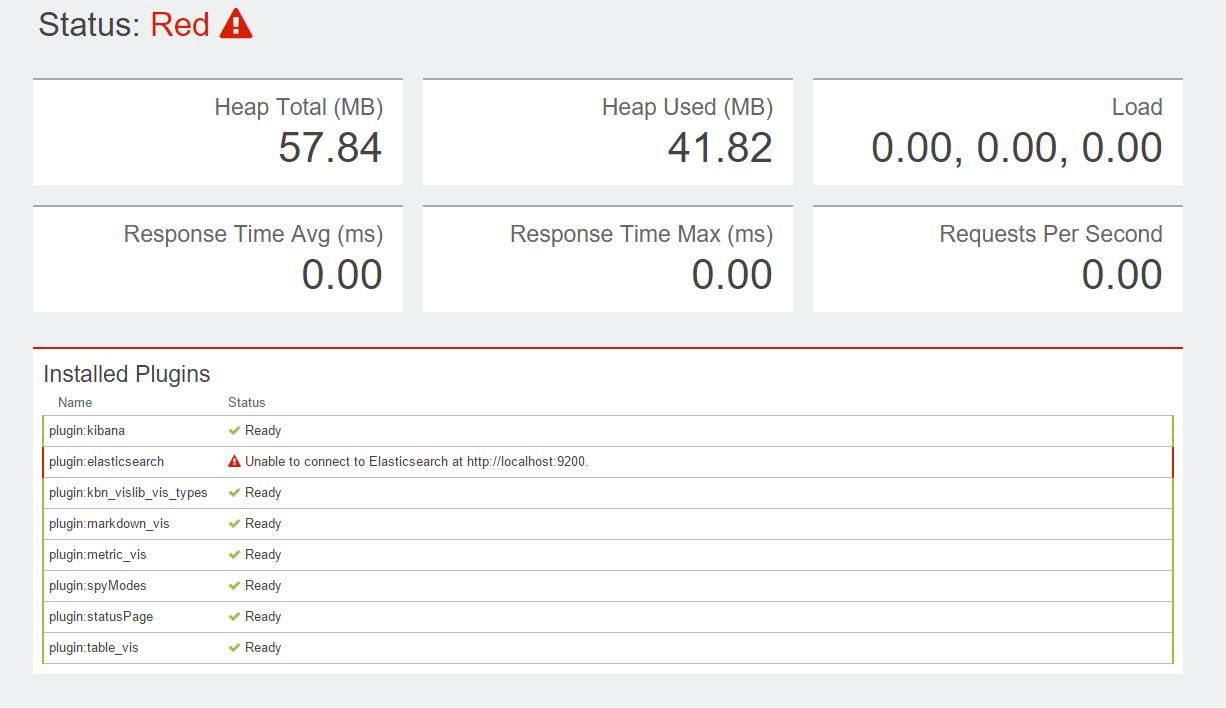
\includegraphics[width=1.0\textwidth]{images/kibana_status}
    \caption[Status serwera Kibana]{
        Status serwera Kibana, źródło: opracowanie własne
    }
    \label{chapter:application_own:plans:monitoring_kibana:picture}
\end{figure}

Autor, poniższej pracy dyplomowej, zaproponował wprowadzenie do projektu \textbf{monasca-agent} nowych komponentów, które
wspierałyby okresowe zbierania metryk z programu Kibana. Pobrane informacje mogłyby służyć do tworzenia
nowych alarmów lub historycznej analizy stanu aplikacji z wykorzystaniem diagramów dostępnych z poziomu komponentu 
\textbf{monasca-ui}. Całość implementacji zawarta byłaby w dwóch, nowych, elementach \textbf{monasca-agent}, które
pozwalałyby na:
\begin{itemize}
    \item[automatyczną detekcję Kibana] - podczas startu \textbf{monasca-agent} uruchamiany jest specjalny algorytm, którego
    celem jest automatyczne wykrycie działających aplikacji. Detekcja odbywa się na tej samej maszynie na której działa 
    \textbf{monasca-agent}. W przypadku stwierdzenie, że wspierane aplikacje są uruchomione, \textbf{monasca-agent} tworzy 
    pliki konfiguracyjne informujące proces kolektora, że powinien on uruchomić dedykowany mini program, który w wyniku
    swojego działania, utworzył by nowe metryki.
    \item[pobieranie metryk] - okresowo Kibana byłaby odpytywana o aktualny stan. Uzyskany dane byłyby transformowane
    na metryki.
\end{itemize}